\section{Background}
%
\label{Sect:Background}

We assume familiarity with ordinary category theory~\cite{MacLane2010}, enriched category theory~\cite{Kelly1982}, and string diagrams~\cite{Selinger_2010}.
In this paper, we adopt the following notation.
\begin{itemize}
\item \textbf{MonCat} is the $2$-category of monoidal categories, lax monoidal functors, and monoidal natural transformations.
\item \textbf{BrMonCat} is the $2$-category of braided monoidal categories, lax monoidal functors, and monoidal natural transformations.
\item For a monoidal category $\mathcal{V}$, $\mathbf{Comon}( \mathcal{V} )$ is the category of comonoids in $\mathcal{V}$, and $\mathbf{CComon}( \mathcal{V} )$ is the sub-category of cocommutative comonoids in $\mathcal{V}$.
\item If $\mathcal{V}$ is a monoidal closed category with $f \in \mathcal{V}( X, Y )$, then we write $[f]$ for the image of $f$ under the isomorphism $\mathcal{V}( X, Y ) \cong \mathcal{V}( \mathbb{I}, [ X, Y ] )$ and $\app_{X,Y}: [ X, Y ] \otimes X \to Y$ for the corresponding evaluation map.
\item If $\mathcal{V}$ is a monoidal category, then $\mathcal{V}\mathbf{Cat}$ is the $2$-category of $\mathcal{V}$-categories, $\mathcal{V}$-natural transformations, and $\mathcal{V}$-functors.
\end{itemize}
We briefly review the key concepts used in this paper.

\vspace{1em}
\noindent
\textbf{Categories of Comonoids}.
%
Let $( \mathcal{V}, \otimes, \mathbb{I}, \alpha, \lambda, \rho )$ be a monoidal category.
We recall the following results from~\cite{Porst01062008}.
If $\mathcal{V}$ is braided monoidal with braiding $\beta$, then $\mathbf{Comon}( \mathcal{V} )$ is a monoidal category with $( P, d, e ) \otimes ( Q, \delta, \epsilon ) := ( P \otimes Q, ( 1 \otimes \beta_{P,Q} \otimes 1 ) \circ d \otimes \delta, e \otimes \epsilon )$ and monoidal unit $( \mathbb{I}, \lambda_{\mathbb{I}}^{-1}, 1_{\mathbb{I}} )$.
The unitors and associator are inherited from $\mathcal{V}$.
Moreover, if $\mathcal{V}$ is symmetric monoidal, then $\mathbf{Comon}( \mathcal{V} )$ is also a symmetric monoidal category.

\vspace{1em}
\noindent
\textbf{Cartesian Monoidal Categories}.
%
A Cartesian monoidal category is a monoidal category $\mathcal{M} = ( \mathcal{V}, \otimes, \mathbb{I}, \alpha, \lambda, \rho )$ in which $\otimes$ is the categorical product and $\mathbb{I}$ is the terminal object.
It follows from~\cite{Fox1976} that if $\mathcal{M}$ is symmetric monoidal, then $\mathcal{M}$ is Cartesian monoidal if and only if $\mathcal{M}$ is isomorphic to $\mathbf{Comon}( \mathcal{V} )$ as a symmetric monoidal category~\cite{Arkor2025}.
Consequently, each object in $\mathcal{M}$ admits a unique comonoid structure.
Theorems of this form are referred to as \emph{Fox's Theorems}.
A similar characterization is given in~\cite{HeunenVicary2019}.
The category $\mathcal{M}$ is said to have \emph{uniform deleting} if there exists a natural transformation $e: \mathcal{V} \Rightarrow \mathbb{I}$ satisfying $e_{\mathbb{I}} = \lambda_{\mathbb{I}}$ and $e_{A \otimes B} = \lambda_{\mathbb{I}} \circ ( e_A \otimes e_B )$ for each $A \in \mathcal{V}_0$ and $B \in \mathcal{V}_0$.
The category $\mathcal{M}$ is said to have \emph{uniform copying} if $\mathcal{M}$ is symmetric monoidal and there exists a natural transformation $\Delta: \mathcal{V} \Rightarrow \mathcal{V} \otimes \mathcal{V}$ such that $\Delta_{\mathbb{I}} = \rho_{\mathbb{I}}$ and the following equation of diagrams holds for each $A \in \mathcal{V}_0$ and $B \in \mathcal{V}_0$ (of course, $\lambda_{\mathbb{I}} = \rho_{\mathbb{I}}$~\cite{Kelly1964}).
\begin{equation}
    \label{Eqn:MonoidProd}
    \Delta_{P \otimes Q}
    =
    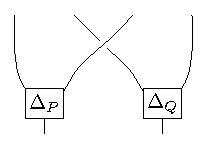
\includegraphics[valign=c,scale=0.85]{figs/special/monoid_product.pdf}
\end{equation}

\begin{prop}[\cite{HeunenVicary2019}]
    \label{Prop:Cartesian}
    A monoidal category $\mathcal{M}$ is Cartesian monoidal if and only if $\mathcal{M}$ has uniform deleting $e: \mathcal{V} \to \mathbb{I}$ and uniform copying $\Delta: \mathcal{V} \to \mathcal{V} \otimes \mathcal{V}$ such that $( A, \Delta_A, e_A )$ is a comonoid object in $\mathcal{M}$ for each $A \in \mathcal{V}_0$.
\end{prop}

\vspace{1em}
\noindent
\textbf{Dagger Categories}.
%
A \emph{dagger structure}~\cite{Selinger2007} on a category $\mathcal{C}$ is a functor $\dagger: \mathcal{C} \to \mathcal{C}^{\text{op}}$ such that $X^\dagger = X$ for each $X \in \mathcal{C}_0$ and $( f^\dagger )^\dagger = f$ for each $f \in \mathcal{C}_1$.
If $( \dagger )$ is dagger structure on $\mathcal{C}$ and $( \ddagger )$ is a dagger structure on $\mathcal{D}$, then $F: \mathcal{C} \to \mathcal{D}$ is a dagger-functor when $F( f^\dagger ) = F( f )^\ddagger$ for all $f \in \mathcal{C}( X, Y )$.
A \emph{monoidal dagger structure}~\cite{Selinger2007,Selinger_2010} on a monoidal category $( \mathcal{V}, \otimes, \mathbb{I}, \alpha, \lambda, \rho )$ is a dagger structure $( \dagger )$ on $\mathcal{V}$ such that the following properties hold.
\begin{itemize}
\item If $f \in \mathcal{V}_1$ and $g \in \mathcal{V}_1$, then $( f \otimes g )^\dagger = f^\dagger \otimes g^\dagger$.
\item If $X \in \mathcal{C}_0$, $Y \in \mathcal{C}_0$, and $Z \in \mathcal{C}_0$, then $\alpha_{X,Y,Z}^\dagger = \alpha_{X,Y,Z}^{-1}$.
\item If $X \in \mathcal{C}_0$, then $\lambda_X^\dagger = \lambda_X^{-1}$ and $\rho_X^\dagger = \rho_X^{-1}$.
\end{itemize}
A \emph{vertical reflection} of a string diagram reflects the diagram vertically while replacing each morphism $f$ with its mirror image $f^\dagger$.
If $\dagger$ is a monoidal dagger structure, then vertical reflections respect the equality of string diagrams~\cite{Selinger_2010}.
In this case $( P, m ,e )$ is a monoid in $\mathcal{V}$ if and only if $( P, m^\dagger, e^\dagger )$ is a comonoid in $\mathcal{V}$.
In a monoidal closed category with a monoidal dagger structure, $\app_{Y,X} \circ ( [f^\dagger] \otimes 1_Y ) = ( [f]^\dagger \otimes 1_X ) \circ \app_{X,Y}^\dagger$.

\vspace{1em}
\noindent
\textbf{Enriched Categories}.
%
We write $\mathcal{C}^{\mathcal{V}}$ for a category enriched over $\mathcal{V}$ and $\mathcal{C}$ for the underlying category.
If $( F, \eta, \epsilon ): \mathcal{V} \to \mathcal{W}$ is a lax monoidal functor, then there exists a \emph{base change} functor $F_{*}: \mathcal{V}\mathbf{Cat} \to \mathcal{W}\mathbf{Cat}$~\cite{Kelly1982}.
If $\mathcal{C}^{\mathcal{V}}$ has enriched composition $M$ and enriched identity $1_X$, then $F_*( \mathcal{C}^{\mathcal{V}} )$ will have enriched composition $F( M ) \circ \eta$ and enriched identity $1_X \circ \epsilon$.
We will write $( \mathcal{C}^{\mathcal{V}}, \mathbb{I}, \otimes^{\mathcal{V}}, \alpha^{\mathcal{V}}, \lambda^{\mathcal{V}}, \rho^{\mathcal{V}} )$ for a $\mathcal{V}$-enriched monoidal category and $( \mathcal{C}, \mathbb{I}, \otimes, \alpha, \lambda, \rho )$ for the underlying monoidal category.
Since $\mathcal{V}$-enriched monoidal categories are pseudomonoids in $\mathcal{V}\mathbf{Cat}$, $F_*$ also sends $\mathcal{V}$-enriched monoidal categories to $\mathcal{W}$-enriched monoidal categories, provided $F$ is braided~\cite{Cruttwell2008}.
When $\mathcal{V}$ is symmetric monoidal, it is straight-forward to show that $F_*$ also preserves braided (resp. symmetric) pseudomonoids in $\mathcal{V}\mathbf{Cat}$, corresponding to $\mathcal{V}$-enriched braided (resp. symmetric) monoidal categories (see the supplementary material for more details).
When $\mathcal{V}$ is monoidal closed, it can be shown that $\mathcal{V}$ is the underlying category of some $\mathcal{V}$-enriched category whose hom-objects are the internal homs and whose composition is defined using the hom-tensor adjunction~\cite{Kelly1982}.
Moreover, if $\mathcal{V}$ is braided monoidal closed, then the monoidal product on $\mathcal{V}$ also translates to the $\mathcal{V}$-enriched setting (see~\cite{10.1093/imrn/rnx217} for a special case).
Throughout this paper, we will reason about enriched categories via string diagrams, as in~\cite{Wesley2024} and~\cite{10.1093/imrn/rnx217}.

\begin{figure}[t]
    \begin{subfigure}[b]{0.5\textwidth}
        \centering
        \begin{equation*}
            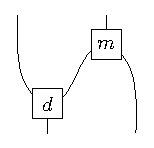
\includegraphics[valign=c,scale=0.85]{figs/background/frob_law_2.pdf}
            =
            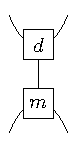
\includegraphics[valign=c,scale=0.85]{figs/background/frob_law_1.pdf}
            =
            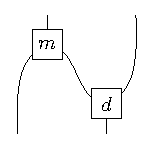
\includegraphics[valign=c,scale=0.85]{figs/background/frob_law_3.pdf}
        \end{equation*}
        \caption{The extended Frobenius law.}
        \label{Fig:Frob:Law}
    \end{subfigure}
    \begin{subfigure}[b]{0.22\textwidth}
        \centering
        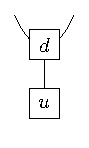
\includegraphics[valign=c,scale=0.85]{figs/background/frob_unit.pdf}
        \caption{The unit $\eta$.}
        \label{Fig:Frob:Unit}
    \end{subfigure}
    \begin{subfigure}[b]{0.22\textwidth}
        \centering
        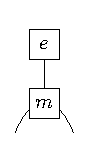
\includegraphics[valign=c,scale=0.85]{figs/background/frob_counit.pdf}
        \caption{The counit $\epsilon$.}
        \label{Fig:Frob:Counit}
    \end{subfigure}
    \caption{Structure of a Frobenius algebra $A = ( P, m, d, u, e )$ with $P \vdash P$.}
        \label{Fig:Frob}
\end{figure}

\vspace{1em}
\noindent
\textbf{Controlled Operations}.
%
We write $\{ \ket{0}, \ket{1}, \ldots, \ket{n-1} \}$ for the standard basis in $\mathbb{C}^n$, $I_n$ for the $n \times n$ identity matrix, and $\bra{j}$ for the dual basis vector to $\ket{j}$.
Given a unitary transformation $U: \mathbb{C}^n \to \mathbb{C}^n$, we write $C( U ) = \ket{0} \bra{0} \otimes I_n + \ket{1} \bra{1} \otimes U$ for the \emph{standard controlled version of $U$}~\cite{NielsenChuang2010}.
This definition can be stated more generally in terms of special commutative $\dagger$-Frobenius structures, as outlined in~\cite{HeunenVicary2019}.
Recall that a \emph{Frobenius structure} in a braided monoidal category $\mathcal{V}$ is an object $P \in \mathcal{V}_0$ equipped with a monoid structure $( P, m, u )$ and a comonoid structure $( P, d, e )$ satisfying the equation in~\cref{Fig:Frob:Law}.
It follows that if $P$ admits a Frobenius structure, then $P$ is self-adjoint as in~\cref{Fig:Frob}.
Moreover, if $P$ is self-adjoint, then $( P, 1_P \otimes \eta \otimes 1_P, \epsilon )$ is a comonoid, referred to as the \emph{pair-of-pants} comonoid in~\cite{HeunenVicary2019}.
It follows from this adjunction that the comonoid $( P, d, e )$ is uniquely determined by the choice of monoid $( P, m, u )$ and the choice of counit $e$.

\begin{prop}[\cite{HeunenVicary2019}]
    \label{Prop:NonDegenForm}
    If $( P, m, u )$ is a monoid in $\mathcal{V}$, then there exists a bijective correspondence between the following structures.
    \begin{enumerate}
    \item Comonoids $( P, d, e )$ making $( P, m, d, u, e )$ a Frobenius algebra.
    \item Morphisms $e: P \to \mathbb{I}$ making $e \circ m$ the counit of an adjunction $P \vdash P$.
    \end{enumerate}
    Given such an $e: P \to \mathbb{I}$ and unit $\eta$, the comultiplication is defined as follows.
    \begin{equation*}
        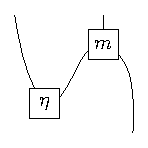
\includegraphics[valign=c,scale=0.85]{figs/background/comult_def_1.pdf}
        =
        d
        =
        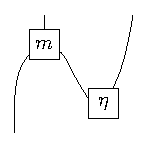
\includegraphics[valign=c,scale=0.85]{figs/background/comult_def_2.pdf}
    \end{equation*}
\end{prop}

If $( P, m, u )$ is commutative and $( P, d, e )$ is cocommutative, then $( P, m, d, u, e )$ is a commutative Frobenius algebra.
If $( \dagger )$ is a dagger-structure for $\mathcal{V}$ and $( P, d, e ) = ( P, m^\dagger, u^\dagger )$, then $A$ is $\dagger$-Frobenius algebra.
If $d \circ m = 1_P$, then $A$ is a special Frobenius algebra.
This yields a categorical characterization of orthogonal bases.

\begin{defi}[Copyable State~\cite{Coecke2012}]
    The \emph{copyable states} of a Frobenius algebra $( P, m, d, u, e )$ in $\mathcal{V}$ are the generalized elements $x \in \mathcal{V}( \mathbb{I}, P )$ such that $d \circ x = x \otimes x \circ \lambda_X^{-1}$.
\end{defi}

\begin{prop}[\cite{Coecke2012}]
    \label{Prop:BasisComonoid}
    Let $\mathcal{V} = \mathbb{C}\mathbf{FVect}$ be the category of finite-dimensional complex vector spaces, $\dagger: \mathcal{V} \to \mathcal{V}^\text{op}$ be the conjugate transpose functor, and $A = ( P, m, d, u, e )$ be a Frobenius algebra in $\mathcal{V}$.
    Then the following statements are equivalent.
    \begin{enumerate}
    \item $A$ is a special commutative $\dagger$-Frobenius algebra.
    \item The copyable states of $A$ form an orthonormal basis for $P$.
    \end{enumerate}
    Moreover, if $\mathcal{B} = \{ \ket{b_1}, \ket{b_2}, \ldots, \ket{b_n} \}$ is an orthonormal basis for $P$, then $\mathcal{B}$ consists of the copyable states for a special commutative $\dagger$-Frobenius algebra with comultiplication defined linearly by $d: \ket{b_j} \mapsto \ket{b_j} \otimes \ket{b_j}$ with $e = \sum_{j=1}^n \bra{b_j}$.
\end{prop}

As in linear algebra, it is possible to consider modules of monoid objects.
The free modules of a special commutative $\dagger$-Frobenius algebra $A$ correspond to measuring the monoid object with respect to the defining basis of $A$.
The module homomorphisms of these free modules then correspond to generalized controlled operations with respect to the defining basis.
In~\cite{HeunenVicary2019}, controlled operations are generalized further, to include module homomorphisms of all $\dagger$-modules over special commutative $\dagger$-Frobenius algebras.

\begin{defi}[Module]
    Let $M = ( P, m, u )$ be a monoid in $\mathcal{V}$.
    An $M$-module is an object $X \in \mathcal{V}_0$ with a choice of morphism $\mu \in \mathcal{V}( P \otimes X, X )$ satisfying the following equations.
    \begin{align*}
        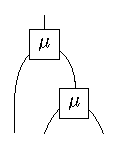
\includegraphics[valign=c,scale=0.85]{figs/background/modmult_lhs.pdf}
        &=
        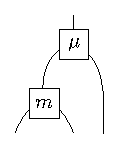
\includegraphics[valign=c,scale=0.85]{figs/background/modmult_rhs.pdf}
        &
        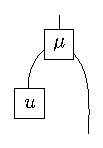
\includegraphics[valign=c,scale=0.85]{figs/background/modunit_lhs.pdf}
        &=
        1_X
    \end{align*}
    If there exists some object $Y \in \mathcal{V}_0$ such that $X = P \otimes Y$ and $\mu = m \otimes 1_Y$, then $( X, \mu )$ is said to be a free $M$-module.
    The dual notion to an $M$-module is an $M$-comodule.
\end{defi}

\begin{defi}[Module Homomorphism]
    Let $M = ( P, m, u )$ be a monoid in $\mathcal{V}$ with $M$-modules $( X, \mu )$ and $( Y, \nu )$.
    An $M$-module homomorphism from $( X, \mu )$ to $( Y, \nu )$ is a morphism $f \in \mathcal{V}( X, Y )$ such that $f \circ \nu = \mu \circ ( 1_P \otimes f )$.
\end{defi}

More recently, control functors have been introduced, which generalize the endofunctor that maps each unitary $U$ to its controlled version $C( U )$~\cite{Delorme2026}.
In this paper we consider a generalization of control functors to braided monoidal categories.
Let $( \mathcal{C}, \otimes, \mathbb{I}, \beta, \alpha, \lambda, \rho )$ be a braided monoidal category with sub-category $\mathcal{C}_{\mathbf{Endo}}$ of endomorphisms.
A \emph{control functor} is an ordinary functor $C: \mathcal{C}_{\mathbf{Endo}} \to \mathcal{C}_{\mathbf{Endo}}$ equipped with an object $P \in \mathcal{C}_0$ such that $F_0( X ) = P \otimes X$ subject to the following axioms.
\begin{itemize}
\item \textbf{Tensor Axiom}.
      If $f \in \mathcal{C}( X, X )$ and $Z \in \mathcal{C}_0$, then $C( f \otimes 1_Z ) = C( f ) \otimes 1_Z$.
\item \textbf{Target Symmetry Axiom}.
      If $X, Y, Z, W \in \mathcal{V}_0$, $f \in \mathcal{C}( X \otimes Y \otimes Z \otimes W, X \otimes Y \otimes Z \otimes W )$ and $\sigma = 1_X \otimes \beta_{Y,Z} \otimes 1_W$, then $C( \sigma^{-1} \circ f \circ \sigma ) = ( 1_P \otimes \sigma^{-1} ) \circ C( f ) \circ ( 1_P \otimes \sigma )$.
\item \textbf{Control Symmetry Axiom}.
      If $f \in \mathcal{C}( X, X )$, then $( \beta_{P,P} \otimes 1_X ) \circ C( f ) = ( \beta_{P,P} \otimes 1_X ) \circ C( f )$.
\end{itemize}
A control functor is \emph{$( u, v )$-pointed} if there exists $u \in \mathcal{C}( \mathbb{I}, P )$ and $v \in \mathcal{C}( \mathbb{I}, P )$ which satisfy the \textbf{Activation Axiom}: $C( f ) \circ ( u \otimes 1_X ) = u \otimes 1_X$ and $C( f ) \circ ( v \otimes 1_X ) = v \otimes f$ for each $f \in \mathcal{C}( X, X )$.
A control functor is \emph{conguated} if it satisfies the \textbf{Conjugation Axiom}: $C( h \circ g \circ f ) = ( 1_P \otimes h ) \circ C( g ) \circ ( 1_P \otimes f )$ for all $f \in \mathcal{C}( X, Y )$,  $g \in \mathcal{C}( Y, Y )$, and $h \in \mathcal{C}( Y, X )$ satisfying $h \circ f = 1_X$.
A $\dagger$-control functor is a control functor that is also a dagger-endofunctor.
